\documentclass[10pt,a4paper]{report}
\usepackage[utf8]{inputenc}
\usepackage[T1]{fontenc}
\usepackage{amsmath}
\usepackage{amsfonts}
\usepackage{amssymb}
\usepackage{graphicx}
\usepackage{caption}
\usepackage{subcaption}
\usepackage{algorithm2e}
\usepackage{algpseudocode}
\usepackage{amsmath}
\RestyleAlgo{ruled}
\begin{document}
	
\subsection{Geometria}

\subsubsection{Asa}

A asa é definida a partir de 39 parâmetros mostrados na Tabela \ref{tab:wing_parameters}.

\begin{table}[h!]
	\centering
	\caption{Parâmetros necessários para definir a forma da asa.}
	\begin{tabular}{p{3cm}p{8cm}}
		Parâmetros & Ddescrição \\
		\hline
		{$l_{i}, \hspace{0.1cm} i \hspace{0.1cm} \epsilon \hspace{0.1cm} [0, \hspace{0.1cm} 3]$} & Posição e comprimentos que representam a estrutura esquelética da ave. \\
		{$\theta_{i}, \hspace{0.1cm} i \hspace{0.1cm} \epsilon \hspace{0.1cm} [0, \hspace{0.1cm} 7]$} & Ângulo de rotação das articulações. \\
		{$h_{i}, \hspace{0.1cm} i \hspace{0.1cm} \epsilon \hspace{0.1cm} [1, \hspace{0.1cm} 7]$} & Comprimentos para definir os pontos contidos nas curvas. \\
		{$\delta_{i}, \hspace{0.1cm} i \hspace{0.1cm} \epsilon \hspace{0.1cm} [1, \hspace{0.1cm} 10]$} & Número entre 0 e 1 que definem a posição dos pontos de auxiliares. \\
		{$foils_{i}, \hspace{0.1cm} i \hspace{0.1cm} \epsilon \hspace{0.1cm} [1, \hspace{0.1cm} 3]$} &  Pontos de 3 perfis aerodinâmicos, na raíz da asa, no meio e na ponta. \\
		\hline
	\end{tabular}
	\label{tab:wing_parameters}
\end{table}

\textbf{Rotação das Articulações}

O movimento das asas são definidos a partir da rotação nas articulações mostradas na Figura \ref{fig:geo_wing_sections_rotation}. As seções 1, 2 e 3, referentes aos comprimentos {$l_{1}$}, {$l_{2}$} e {$l_{3}$}, foram definidas considerando a estrutura esquelética das aves, referente ao úmero, rádio/ulna e metacarpos respectivamente.

\begin{figure}[h!]
	\centering
	\caption{Seções da asa e seus sistemas de coordenadas.}
	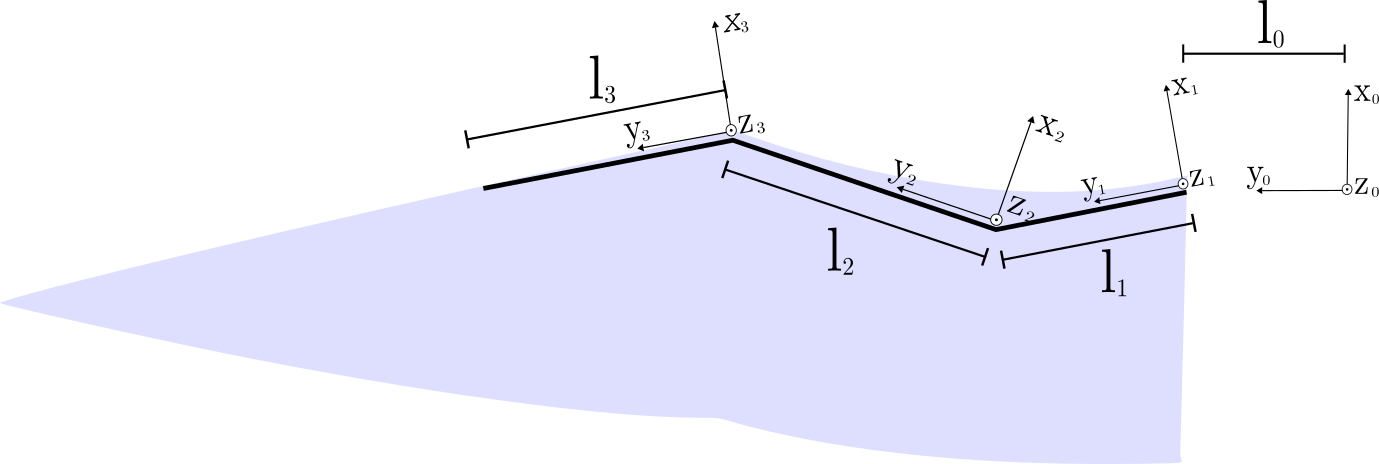
\includegraphics[width=1.0\textwidth]{figures/geo_wing_sections_rotation.png}
	%\source{Lucas Alves, 2022}
	\label{fig:geo_wing_sections_rotation}
\end{figure}

A partir das definições dos sistemas de referência {$(xyz)_{1}$}, {$(xyz)_{2}$} e {$(xyz)_{3}$} na Figura \ref{fig:geo_wing_sections_rotation}, são definidos 14 ângulos de rotação, 7 de cada lado da asa, como mostrado abaixo. O subescrito {$e$} e {$d$} representam o valor do lado esquerdo e direito da asa respectivamente.

\begin{enumerate}
	
	\item Seção 1: a base da seção 1 corresponde à articulação do ombro e pode sofrer rotação em torno dos 3 eixos, referentes aos ângulos {$\theta_{1}$}, {$\theta_{2}$} e {$\theta_{3}$}. Assumindo que inicialmente os vetores unitários {$\hat{x}_{1}$}, {$\hat{y}_{1}$} e {$\hat{z}_{1}$} coincidem com a base do sistema {$(xyz)_{0}$}, as rotações do lado esquerdo da asa são {$\theta_{1_{e}}$}, {$\theta_{2_{e}}$} e {$\theta_{3_{e}}$} em torno de {$\hat{x}_{1_{e}}$}, -{$\hat{y}_{1_{e}}$} e {$\hat{z}_{1_{e}}$} respectivamente. Do lado direito as rotações são em torno dos eixos, -{$\hat{x}_{1_{d}}$}, -{$\hat{y}_{1_{d}}$} e -{$\hat{z}_{1_{d}}$}, e os ângulos são {$\theta_{1_{d}}$}, {$\theta_{2_{d}}$} e {$\theta_{3_{d}}$} respectivamente. Os ângulos são rotacionados em torno dos eixos na ordem {$\hat{y}_{1}$}, {$\hat{x}_{1}$} e {$\hat{z}_{1}$}.
	
	\item Seção 2: a base da segunda seção corresponde à articulação do cotovelo e pode sofrer rotação em torno de 2 eixos, {$\hat{y}_{2}$} e {$\hat{z}_{2}$}, referentes aos ângulos {$\theta_{4}$} e {$\theta_{5}$}. A rotação em torno de {$\hat{y}_{2}$} não é aplicada em toda a seção, mas varia, começando de {$0.0$} na base, até o valor máximo na ponta, como ocorre no antebraço humano. Já o ângulo {$\theta_{5}$} pode assumir apenas valores positivos, uma restrição causada pela articulação. Por fim, as rotações do lado esquerdo da asa, {$\theta_{4_{e}}$} e {$\theta_{5_{e}}$}, ocorrem em torno dos eixos -{$\hat{y}_{2_{e}}$} e -{$\hat{z}_{2_{e}}$}. Já do lado direito, os eixos são -{$\hat{y}_{2_{d}}$} e {$\hat{z}_{2_{d}}$}. Os ângulos são rotacionados em torno dos eixos na ordem {$\hat{z}_{2}$} e {$\hat{y}_{2}$}.
	
	\item Seção 3: a base da terceira seção corresponde à articulação da mão e pode sofrer rotação em torno dos eixos {$\hat{x}_{3}$} e {$\hat{z}_{3}$}, referentes aos ângulos {$\theta_{6}$} e {$\theta_{7}$}. Do lado esquerdo as rotação ocorrem em torno dos eixos -{$\hat{x_{e}}_{3}$} e {$\hat{z}_{3_{e}}$} e, do lado direito {$\hat{x_{e}}_{3}$} e -{$\hat{z}_{3_{e}}$}. Os ângulos são rotacionados em torno dos eixos na ordem {$\hat{x}_{3}$} e {$\hat{z}_{3}$}.
	
\end{enumerate}

\textbf{Contorno}

A Figura \ref{fig:geo_wing_points} mostra os pontos de controle necessários para se definir o contorno da asa.

\begin{figure}[h!]
	\centering
	\caption{Pontos necessários para determinar o contorno da asa. Os pontos verdes estão contidos no contorno, os vermelhos são pontos de controle para determinar as curvas de Bézier e os azuis são pontos auxiliares.}
	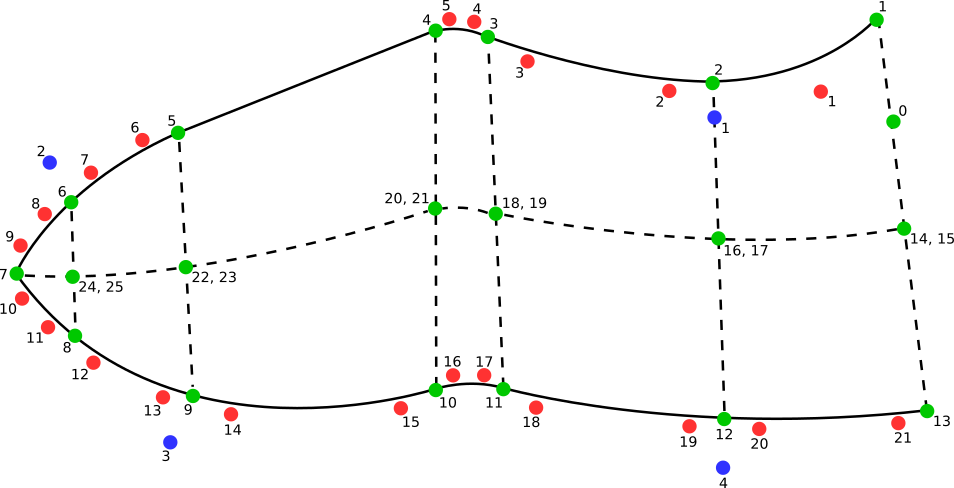
\includegraphics[width=1.0\textwidth]{figures/geo_wing_points.png}
	%\source{Lucas Alves, 2022}
	\label{fig:geo_wing_points}
\end{figure}

\textbf{Pontos: {$\boldsymbol{l_{1}, \hspace{0.1cm} l_{2} \hspace{0.1cm} e \hspace{0.1cm} l_{3}}$}}

\begin{equation}
\vec{l}_{1} = \vec{p}_{0} + l_{1} \hat{y}_{1}
\label{eq:l1}
\end{equation}

\begin{equation}
\vec{l}_{2} = \vec{l}_{1} + l_{2} \hat{y}_{2}
\label{eq:l2}
\end{equation}

\begin{equation}
\vec{l}_{3} = \vec{l}_{2} + l_{3} \hat{y}_{3}
\label{eq:l3}
\end{equation}

\textbf{Ponto: {$\boldsymbol{\vec{p}_{0}}$}}

\begin{equation}
\vec{p}_{0} = l_{0} \hat{y}_{0}
\label{eq:p0}
\end{equation}

\textbf{Ponto: {$\boldsymbol{\vec{p}_{1}}$}}

\begin{equation}
\vec{p}_{1} = \vec{p}_{0} + q(\theta_{2}, -\hat{y}_{0}) q(\theta_{0}, \hat{z}_{0}) (h_{1} \hat{x}_{0}) q'(\theta_{0}, \hat{z}_{0}) q'(\theta_{2}, -\hat{y}_{0})
\label{eq:p1}
\end{equation}

\textbf{Ponto: {$\boldsymbol{\vec{p}_{2}}$}}

\begin{equation}
\vec{p}_{2} = \frac{\vec{p}_{1} + 2 \vec{c}_{aux_{1}} + \vec{p'}_{3}}{4}
\label{eq:p2}
\end{equation}

\begin{equation}
\vec{c}_{aux_{1}} = \vec{l}_{1} + \delta_{1} \frac{|| (\vec{p}_{0} + l_{1} \hat{y}_{1} - \vec{p}_{1}) \times (\vec{p}_{0} + l_{1} \hat{y}_{1} - \vec{p}_{3}) ||}{|| \vec{p}_{3} - \vec{p}_{1} ||} unary(\hat{x}_{1} + \hat{x}_{base_{2}})
\label{eq:c_aux_1}
\end{equation}

\begin{equation}
\vec{p'}_{3} = \vec{l}_{2} - h_{2} \hat{y}_{2} + h_{3} \hat{x}_{base_{2}}
\label{eq:p3_line}
\end{equation}

\textbf{Ponto: {$\boldsymbol{\vec{p}_{3}}$}}

\begin{equation}
\vec{p}_{3} = \vec{l}_{2} - h_{2} \hat{y}_{2} + h_{3} \hat{x}_{Tip_{2}}
\label{eq:p3}
\end{equation}

\textbf{Ponto: {$\boldsymbol{\vec{p}_{4}}$}}

\begin{equation}
\vec{p}_{4} = \vec{l}_{2} + h_{2} \hat{y}_{3} + h_{3} \hat{x}_{3}
\label{eq:p4}
\end{equation}

\textbf{Ponto: {$\boldsymbol{\vec{p}_{5}}$}}

\begin{equation}
\vec{p}_{5} = \vec{l}_{3} + h_{3} \hat{x}_{3}
\label{eq:p5}
\end{equation}

\textbf{Ponto: {$\boldsymbol{\vec{p}_{6}}$}}

\begin{equation}
\vec{p}_{6} = (1 - (1 - \epsilon_{1}))^{2} \vec{p}_{5} + 2 (1 - \epsilon_{1}) (1 - (1 - \epsilon_{1})) \vec{c}_{aux_{2}} + (1 - \epsilon_{1})^{2} \vec{p}_{7}
\label{eq:p6}
\end{equation}

\begin{equation}
\vec{c}_{aux_{2}} = \vec{p}_{5} + \delta_{2} (\hat{y}_{3} \cdot (\vec{p}_{7} - \vec{p}_{5})) \hat{y}_{3}
\label{eq:wing_cp_16}
\end{equation}

\textbf{Ponto: {$\boldsymbol{\vec{p}_{7}}$}}

\begin{equation}
\vec{p}_{7} = \vec{p}_{5} - h_{4} \hat{x}_{3} + h_{5} \hat{y}_{3}
\label{eq:p7}
\end{equation}

\textbf{Ponto: {$\boldsymbol{\vec{p}_{8}}$}}

\begin{equation}
\vec{p}_{8} = (1 - \epsilon_{1})^{2} \vec{p}_{7} + 2 \epsilon_{1} (1 - \epsilon_{1}) \vec{c}_{aux_{3}} + \epsilon_{1}^{2} \vec{p}_{10}
\label{eq:p8}
\end{equation}

\begin{equation}
\vec{c}_{aux_{3}} = 0.5 (\vec{p}_{6} + \vec{p}_{7}) + 0.5 \delta_{3} (\vec{p}_{6} - \vec{p}_{7}) + 0.5 \delta_{4} (\hat{z}_{3} \times (\vec{p}_{6} - \vec{p}_{7}))
\label{eq:c_aux_3}
\end{equation}

\textbf{Ponto: {$\boldsymbol{\vec{p}_{9}}$}}

\begin{equation}
\vec{p}_{9} = (1 - \epsilon_{2})^{2} \vec{p}_{7} + 2 \epsilon_{2} (1 - \epsilon_{2}) \vec{c}_{aux_{3}} + \epsilon_{2}^{2} \vec{p}_{10}
\label{eq:p9}
\end{equation}

\textbf{Ponto: {$\boldsymbol{\vec{p}_{10}}$}}

\begin{equation}
\vec{p}_{10} = \vec{p}_{4} - h_{6} unary(\hat{x}_{tip_{2}} + \hat{x}_{3})
\label{eq:p10}
\end{equation}

\textbf{Ponto: {$\boldsymbol{\vec{p}_{11}}$}}

\begin{equation}
\vec{p}_{11} = \vec{p}_{3} - h_{6} unary(\hat{x}_{tip_{2}} + \hat{x}_{3})
\label{eq:p11}
\end{equation}

\textbf{Ponto: {$\boldsymbol{\vec{p}_{12}}$}}

\begin{equation}
\vec{p}_{12} = \frac{\vec{p}_{11} + 2 \vec{c}_{aux_{4}} + \vec{p}_{13}}{4}
\label{eq:p12}
\end{equation}

\begin{multline}
\vec{c}_{aux_{4}} = 0.5 (\vec{p}_{7} + \vec{p}_{8}) + 0.5 \delta_{5} (\vec{p}_{7} - \vec{p}_{8}) + \\ \delta_{6} || \vec{p}_{7} - \vec{p}_{8} || unary( (\hat{z}_{tip_{2}} + \hat{z}_{base_{2}}) \times (\vec{p}_{7} - \vec{p}_{8}))
\label{eq:c_aux_4}
\end{multline}

\textbf{Ponto: {$\boldsymbol{\vec{p}_{13}}$}}

\begin{equation}
\vec{p}_{13} = \vec{p}_{0} + q(\theta_{2}, -\hat{y}_{0}) q(\theta_{0}, \hat{z}_{0}) (- h_{7} \hat{x}_{0}) q'(\theta_{0}, \hat{z}_{0}) q'(\theta_{2}, -\hat{y}_{0})
\label{eq:p13}
\end{equation}

\textbf{Pontos: {$\boldsymbol{\vec{p}_{14} \hspace{0.2cm} e \hspace{0.2cm} \vec{p}_{15}}$}}

\begin{equation}
\vec{p}_{14} = 0
\label{eq:p14}
\end{equation}

\begin{equation}
\vec{p}_{15} = 0
\label{eq:p15}
\end{equation}

\textbf{Pontos: {$\boldsymbol{\vec{p}_{16} \hspace{0.2cm} e \hspace{0.2cm} \vec{p}_{17}}$}}

\begin{equation}
\vec{p}_{16} = 0
\label{eq:p16}
\end{equation}

\begin{equation}
\vec{p}_{17} = 0
\label{eq:p17}
\end{equation}

\textbf{Pontos: {$\boldsymbol{\vec{p}_{18} \hspace{0.2cm} e \hspace{0.2cm} \vec{p}_{19}}$}}

\begin{equation}
\vec{p}_{18} = 0
\label{eq:p18}
\end{equation}

\begin{equation}
\vec{p}_{19} = 0
\label{eq:p19}
\end{equation}

\textbf{Pontos: {$\boldsymbol{\vec{p}_{20} \hspace{0.2cm} e \hspace{0.2cm} \vec{p}_{21}}$}}

\begin{equation}
\vec{p}_{20} = 0
\label{eq:p20}
\end{equation}

\begin{equation}
\vec{p}_{21} = 0
\label{eq:p21}
\end{equation}

\textbf{Pontos: {$\boldsymbol{\vec{p}_{22} \hspace{0.2cm} e \hspace{0.2cm} \vec{p}_{23}}$}}

\begin{equation}
\vec{p}_{22} = 0
\label{eq:p22}
\end{equation}

\begin{equation}
\vec{p}_{23} = 0
\label{eq:p23}
\end{equation}

\textbf{Pontos: {$\boldsymbol{\vec{p}_{24} \hspace{0.2cm} e \hspace{0.2cm} \vec{p}_{25}}$}}

\begin{equation}
\vec{p}_{24} = 0
\label{eq:p24}
\end{equation}

\begin{equation}
\vec{p}_{25} = 0
\label{eq:p25}
\end{equation}

\textbf{Ponto: {$\boldsymbol{\vec{c}_{1}}$}}

\begin{equation}
\vec{c}_{1} = arg \hspace{0.2cm} min \hspace{0.2cm} (\vec{f}_{1}(\vec{x}, t) - \vec{f}_{2}(t))^{2}; \hspace{0.2cm}  t \hspace{0.1cm}  \epsilon \hspace{0.1cm}  [0, 1]
\label{eq:c1}
\end{equation}

\begin{equation}
\vec{f}_{1} = (1 - t)^{2} \vec{p}_{1} + 2 t (1 - t) \vec{x} + t^{2} \vec{p}_{2}
\label{eq:f1}
\end{equation}

\begin{equation}
\vec{f}_{2} = (1 - 0.5 t)^{2} \vec{p}_{1} + t (1 - 0.5 t) \vec{c}_{aux_{1}} + (0.5 t)^{2} \vec{p'}_{3}
\label{eq:f2}
\end{equation}

\textbf{Ponto: {$\boldsymbol{\vec{c}_{2}}$}}

\begin{equation}
\vec{c}_{2} = \vec{p}_{2} + \epsilon_{3} ((\vec{p}_{3} - \vec{p}_{2}) \cdot unary(\vec{p}_{3} - \vec{p}_{1})) unary(\vec{p}_{3} - \vec{p}_{1})
\label{eq:c2}
\end{equation}

\textbf{Ponto: {$\boldsymbol{\vec{c}_{3}}$}}

\begin{equation}
\vec{c}_{3} = \vec{p}_{3} + \epsilon_{3} ((\vec{p}_{2} - \vec{p}_{3}) \cdot unary(\vec{p}_{3} - \vec{c}_{4})) unary(\vec{p}_{3} - \vec{c}_{4})
\label{eq:c3}
\end{equation}

\textbf{Ponto: {$\boldsymbol{\vec{c}_{4}}$}}

\begin{equation}
\vec{c}_{4} = \vec{p}_{3} + \epsilon_{4} h_{2} (1 + arccos(-\hat{y}_{2} \cdot \hat{y}_{3})) \hat{y}_{2}
\label{eq:c4}
\end{equation}

\textbf{Ponto: {$\boldsymbol{\vec{c}_{5}}$}}

\begin{equation}
\vec{c}_{5} = \vec{p}_{6} + r_{1} \frac{d \vec{p}_{6}}{dt}
\label{eq:c5}
\end{equation}

\begin{equation}
r_{1} = arg \hspace{0.2cm} min \hspace{0.2cm} \Big( \vec{f}_{3} \big( x, t \big) - \vec{f}_{4} \big( t (1 - \epsilon_{4}) \big) \Big) ^{2}; \hspace{0.2cm}  t \hspace{0.1cm}  \epsilon \hspace{0.1cm}  [0, 1 - \epsilon_{4}]
\label{eq:r1}
\end{equation}

\begin{equation}
\vec{f}_{3}(x, i) = (1 - i)^{2} \vec{p}_{1} + 2 i (1 - i) (\vec{p}_{6} + x \frac{d \vec{p}_{6}}{dt}) + i^{2} \vec{p}_{2}
\label{eq:f3}
\end{equation}

\begin{equation}
\vec{f}_{4}(i) = (1 - i)^{2} \vec{p}_{1} + 2 i (1 - i) \vec{c}_{aux_{1}} + i^{2} \vec{p'}_{3}
\label{eq:f4}
\end{equation}

\textbf{Ponto: {$\boldsymbol{\vec{c}_{6}}$}}

\begin{equation}
\vec{c}_{6} = \vec{p}_{6} + r_{2} \frac{d \vec{p}_{6}}{dt}
\label{eq:c6}
\end{equation}

\begin{equation}
r_{2} = arg \hspace{0.2cm} min \hspace{0.2cm} \Big( \vec{f}_{5} \big( x, t \big) - \vec{f}_{6} \big( 1 + \epsilon_{4}(t - 1) \big) \Big) ^{2}; \hspace{0.2cm}  t \hspace{0.1cm}  \epsilon \hspace{0.1cm}  [1 - \epsilon_{4}, 1]
\label{eq:r2}
\end{equation}

\begin{equation}
\vec{f}_{5}(x, i) = (1 - i)^{2} \vec{p}_{1} + 2 i (1 - i) (\vec{p}_{6} + x \frac{d \vec{p}_{6}}{dt}) + i^{2} \vec{p}_{2}
\label{eq:f5}
\end{equation}

\begin{equation}
\vec{f}_{6}(i) = (1 - i)^{2} \vec{p}_{1} + 2 i (1 - i) \vec{c}_{aux_{1}} + i^{2} \vec{p'}_{3}
\label{eq:f6}
\end{equation}

\textbf{Ponto: {$\boldsymbol{\vec{c}_{7}}$}}

\begin{equation}
\vec{c}_{7} = \vec{p}_{8} + r_{3} \frac{d \vec{p}_{8}}{dt}
\label{eq:c7}
\end{equation}

\begin{equation}
r_{3} = arg \hspace{0.2cm} min \hspace{0.2cm} \Big( \vec{f}_{7} \big( x, t \big) - \vec{f}_{8} \big( \epsilon_{4} t \big) \Big) ^{2}; \hspace{0.2cm}  t \hspace{0.1cm}  \epsilon \hspace{0.1cm}  [0, \epsilon_{4}]
\label{eq:r3}
\end{equation}

\begin{equation}
\vec{f}_{7}(x, i) = (1 - i)^{2} \vec{p}_{1} + 2 i (1 - i) (\vec{p}_{8} + x \frac{d \vec{p}_{8}}{dt}) + i^{2} \vec{p}_{2}
\label{eq:f7}
\end{equation}

\begin{equation}
\vec{f}_{8}(i) = (1 - i)^{2} \vec{p}_{1} + 2 i (1 - i) \vec{c}_{aux_{1}} + i^{2} \vec{p'}_{3}
\label{eq:f8}
\end{equation}

\textbf{Ponto: {$\boldsymbol{\vec{c}_{8}}$}}

\begin{equation}
\vec{c}_{8} = \vec{p}_{8} + r_{4} \frac{d \vec{p}_{8}}{dt}
\label{eq:c8}
\end{equation}

\begin{equation}
r_{4} = arg \hspace{0.2cm} min \hspace{0.2cm} \big( f_{9}(x) - f_{10}(x) \big) ^{2}
\label{eq:r4}
\end{equation}

\begin{equation}
f_{9}(x) = \left| \left| \left( \vec{p}_{8} + x \frac{d \vec{p}_{8}}{dt} - \vec{p}_{9} \right) \cdot \frac{d \vec{p}_{9}}{dt} \right| \right|
\label{eq:f9}
\end{equation}

\begin{equation}
f_{10}(x) = \left| \left| \left( \vec{p}_{8} + x \frac{d \vec{p}_{8}}{dt} - \vec{p}_{9} \right) \right| \right| \hspace{0.1cm} \left| \left| \frac{d \vec{p}_{8}}{dt} \right| \right|
\label{eq:f10}
\end{equation}

\textbf{Ponto: {$\boldsymbol{\vec{c}_{9}}$}}

\begin{equation}
\vec{c}_{9} = \vec{p}_{9} + r_{5} \frac{d \vec{p}_{9}}{dt}
\label{eq:c9}
\end{equation}

\begin{equation}
r_{5} = arg \hspace{0.2cm} min \hspace{0.2cm} \big( f_{11}(x) - f_{12}(x) \big) ^{2}
\label{eq:r5}
\end{equation}

\begin{equation}
f_{11}(x) = \left| \left| \left( \vec{p}_{9} + x \frac{d \vec{p}_{9}}{dt} - \vec{p}_{10} \right) \cdot \frac{d \vec{p}_{10}}{dt} \right| \right|
\label{eq:f11}
\end{equation}

\begin{equation}
f_{12}(x) = \left| \left| \left( \vec{p}_{9} + x \frac{d \vec{p}_{9}}{dt} - \vec{p}_{10} \right) \right| \right| \hspace{0.1cm} \left| \left| \frac{d \vec{p}_{10}}{dt} \right| \right|
\label{eq:f12}
\end{equation}

\textbf{Ponto: {$\boldsymbol{\vec{c}_{10}}$}}

\begin{equation}
\vec{c}_{10} = \vec{p}_{0} + l_{1} \hat{y}_{1} + l_{2} \hat{y}_{2} - h_{6} unary(\hat{x}_{tip_{2}} + \hat{x}_{3})
\label{eq:c10}
\end{equation}

\textbf{Ponto: {$\boldsymbol{\vec{c}_{11}}$}}

\begin{equation}
\vec{c}_{11} = \vec{p}_{11} + r_{6} \frac{d \vec{p}_{11}}{dt}
\label{eq:c11}
\end{equation}

\begin{equation}
r_{6} = arg \hspace{0.2cm} min \hspace{0.2cm} \big( f_{13}(x) - f_{14}(x) \big) ^{2}
\label{eq:r6}
\end{equation}

\begin{equation}
f_{13}(x) = \left| \left| \left( \vec{p}_{11} + x \frac{d \vec{p}_{11}}{dt} - \vec{p}_{12} \right) \cdot \frac{d \vec{p}_{12}}{dt} \right| \right|
\label{eq:f13}
\end{equation}

\begin{equation}
f_{14}(x) = \left| \left| \left( \vec{p}_{11} + x \frac{d \vec{p}_{11}}{dt} - \vec{p}_{12} \right) \right| \right| \hspace{0.1cm} \left| \left| \frac{d \vec{p}_{12}}{dt} \right| \right|
\label{eq:f14}
\end{equation}

\textbf{Ponto: {$\boldsymbol{\vec{c}_{12}}$}}

\begin{equation}
\vec{c}_{12} = \vec{p}_{13} + r_{7} \frac{d \vec{p}_{13}}{dt}
\label{eq:c12}
\end{equation}

\begin{equation}
r_{7} = arg \hspace{0.2cm} min \hspace{0.2cm} \big( f_{15}(x) - f_{16}(x) \big) ^{2}
\label{eq:r7}
\end{equation}

\begin{equation}
f_{15}(x) = \left| \left| \left( \vec{p}_{13} + x \frac{d \vec{p}_{13}}{dt} - \vec{p}_{12} \right) \cdot \frac{d \vec{p}_{12}}{dt} \right| \right|
\label{eq:f15}
\end{equation}

\begin{equation}
f_{16}(x) = \left| \left| \left( \vec{p}_{13} + x \frac{d \vec{p}_{13}}{dt} - \vec{p}_{12} \right) \right| \right| \hspace{0.1cm} \left| \left| \frac{d \vec{p}_{12}}{dt} \right| \right|
\label{eq:f16}
\end{equation}

\end{document}